\documentclass[12pt]{article}
%Gumm{\color{blue}i}|065|=)
\usepackage{amsmath, amsfonts, amssymb}
\usepackage[margin=0.5in]{geometry}
\usepackage{xcolor}
\usepackage{graphicx}
\usepackage{amsmath}
\usepackage{hyperref}

\usepackage{fontspec}
\usepackage{xcolor}

\newcommand{\off}[1]{}
\DeclareMathSizes{20}{30}{20}{18}
\usepackage{tikz}

%\setmainfont[Color=brown]{Linux Libertine}


\title{Reading: Approximate Groups}
\date{}
\begin{document}

\sffamily

\maketitle

{\fontsize{16pt}{16pt}\selectfont 

\noindent   \\ \\
 \textbf{Lemma 2.5.1} Let $G$ be a {\color{red!75!black}arbitrary} group and let $A \subset G$ b a finite subset with $|A^2| \leq K | A|$.  Then $|A^{-1}A|\leq K^2 |A|$ and $|A A^{-1}| \leq K^2|A|$. \\ \\
This is generalization to non-abelian groups, only for $m=1$ and $n=1$ \\ \\
\textbf{Theorem 2.3.1}  Let $G$ be an {\color{yellow!50!black}abelian} group and let $A, B$ be finite subsets of $G$.  
\begin{itemize}
	\item suppose that $|A + B| \leq K |A|$ then $|mA - nA| \leq K^{m+n}|A|$.
	\item if $|A+A| \leq K|A|$ then $|mA - nA| \leq K^{m+n}|A|$.
\end{itemize}
for all non-negatve integers $m,n$. \\ \\
These looking into the axioms of group theory.  There are several instances of group theory that we encounter in other branches of mathemamtics:
\begin{itemize}
\item permutation groups \\ $\text{ABCDE} \to \text{BCDEA} \to \text{CDEAB} \to \text{DEABC} \to \text{EABCD} \to [\dots]$
\item groups of substutions, e.g. 
$x \mapsto 3x + 2y \text{ and }y \mapsto 4x + 3y $
\item groups of transformations of physical objects (e.g. symmetries of square)
\end{itemize}
These symmetries in general were approximate since there was an enormous amount of work move and old the objects in a perfect evenly spaced circle. \\ \\
\textbf{Triangle inequality} Let $U,V,W$ be subsets of a group. There exists an injection:
$$ \phi: U \times V^{-1}W \to UV \times UW $$
In particular if $U,V,W$ are finite then $|U| \times |V^{-1}W| \leq |UV||UW|$. \\ \\ 
We're left wondering why the theorem is formatted in this particular way.  The proof use basic notions of algebra like ``function" an  ``inverse" and ``injection".
\begin{itemize}
\item $v : V^{-1} W \to V$ and $w : V^{-1} W \to W$ under then constraint 
that $x \in V^{-1}W$ leads to $x = v(x)^{-1} w(x)$.  
\item set $\phi(u,x) = (uv(x), uw(x))$.
\item check that $\phi$ is injective
\begin{itemize}
\item $(uv(x))^{-1} (uw(x)) = v(x)^{-1} w(x) = x $ so that $x$ is {\color{red}\textbf{uniquely}} determined by $\phi(u,x)$.  
\item $(uv(x)) v(x)^{-1} = u $ so that $u$ is uniquely determined by $\phi(u,x)$ and $x$.
\end{itemize}
The triangle ineqality has a logarithmic form:
$$ \log \frac{|V^{-1}W|}{|V|^{1/2}|W|^{1/2}} 
\leq \log \frac{|U^{-1}V|}{|U|^{1/2}|V|^{1/2}} + \log \frac{|U^{-1}W|}{|U|^{1/2}|W|^{1/2}}$$
\end{itemize}
Rusza's triangle inequality was appliled with all three set's being identical $U = V = W = A$.  In fact, that's the entire argument. \\ \\
So are have not made any spacifications like $G = \mathbb{Z}^2$ or $G = SU(2)$ or $G = \text{SL}_2(\mathbb{Z}[i])$ or $G = (\text{SL}_2(\mathbb{Z}) \backslash \text{SL}_2(\mathbb{R})[5]$ or anything else.  These were deduced abstractly from our guess on how the notion of multipicaton $\times$ or of how mirrors actually work. \\ \\
\textbf{Counterexample} Let $H$ be a finite group and let $G = H \ast \langle x \rangle$ (which is called the \textbf{free product}) of $H$ with the infinite cyclic group (basically a copy of $\mathbb{Z}$, e.g. how many times we do something).  Let $A = H \cup \langle x \rangle$ (this is called the ``union").  Then 
\begin{itemize}
\item $|A^2| \leq 3 |A|$ and yet
\item $HxH \subseteq A^3$ and $|HxH| = |H|^2 \asymp |A|^2$ these sets have the same number of elements without being the same set.  Their definitions look similar too.
\end{itemize} 
\textbf{08/02} Lemma (\textbf{approximate orbit-stabilizer lemma}) Suppose a group $G$ (not necessarily commutative) acts on a set $X$ and let $A$ be a $K$-approximate subgroup of $G$ for some $K \geq 1$.  For every integer $k \geq 2$ and $x \in X$ we have:
$$ |A| \leq |A \cdot x| \; | \text{Stab}(x) \cap A^k| \leq K^{k+1}|A| $$
\textbf{Example} Find examples of approximate groups in $\text{SL}_3(\mathbb{Z}/p\mathbb{Z})$ or $G = SU(2)$.  What happens when subsets don't have ``perfect" multiplicative structure (e.g. \textit{everything} ) or closure properties. \\ \\
\textbf{Theorem} (Orbit-Stabilizer) Let $G$ be a finite group of permutations of the set $S$.  Then for any $i \in S$ $|G| = | \text{orb}(i)| \times |\text{stab}(i)|$.  \\ \\
We have used the word {\color{red!80!black}\textbf{set}}, we  have a ``set" of permutations (I usually think of them as a \textbf{box} or a \textbf{bag}.  So there's varying levels of fluidity there.  Usually we resort to set theory when objects or collections of objects are hard to picture or describe.  We migtt try again later. \\ \\
\textbf{Example} If I shuffle a deck of cards, I have chosen one of the $52! \approx 10^{68}$ possible arrangements of cards.  There's no way we are looking through each one of those.  If I stir a pot, the obects inside have been \textit{permuted}  yet this is close-but-not-quite to the mathematical definition. \\ \\
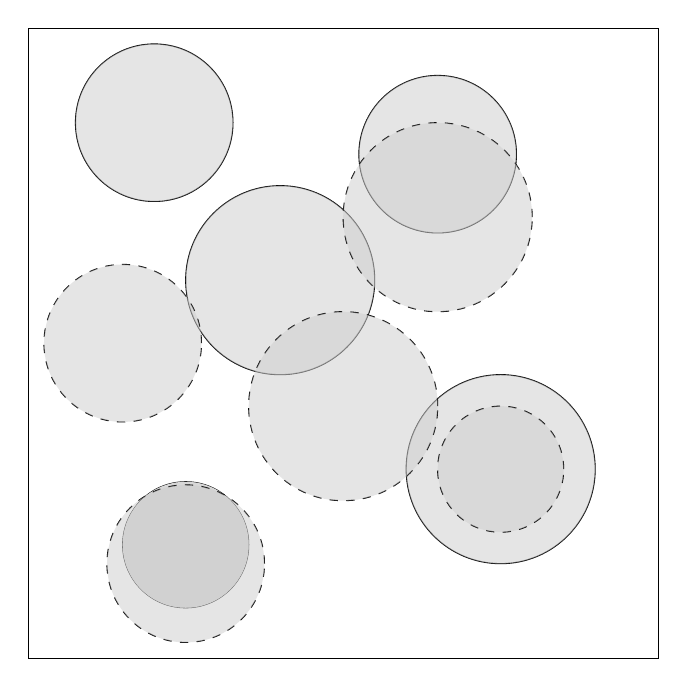
\begin{tikzpicture}[scale=8]
\draw (0,0)--(1,0)--(1,1)--(0,1)--(0,0);

\draw (0.25,0.18) circle (0.1);
\fill[black!10!white] (0.25,0.18) circle (0.1);
\draw (0.75,0.3) circle (0.15);
\draw (0.65,0.8) circle (0.125);
\draw (0.4,0.6) circle (0.15);
\draw (0.2,0.85) circle (0.125);

\fill[black!20!white, opacity=0.5] (0.25,0.18) circle (0.1);
\fill[black!20!white, opacity=0.5] (0.75,0.3) circle (0.15);
\fill[black!20!white, opacity=0.5] (0.65,0.8) circle (0.125);
\fill[black!20!white, opacity=0.5] (0.4,0.6) circle (0.15);
\fill[black!20!white, opacity=0.5] (0.2,0.85) circle (0.125);


\draw[dashed] (0.75,0.3) circle (0.1);
\draw[dashed] (0.65,0.7) circle (0.15);
\draw[dashed] (0.25,0.15) circle (0.125);
\draw[dashed] (0.5,0.4) circle (0.15);
\draw[dashed] (0.15,0.5) circle (0.125);

\fill[black!20!white, opacity=0.5] (0.75,0.3) circle (0.1);
\fill[black!20!white, opacity=0.5] (0.65,0.7) circle (0.15);
\fill[black!20!white, opacity=0.5] (0.25,0.15) circle (0.125);
\fill[black!20!white, opacity=0.5] (0.5,0.4) circle (0.15);
\fill[black!20!white, opacity=0.5] (0.15,0.5) circle (0.125);

\end{tikzpicture}
Once we draw this picture it's not possible to tell which object moved first, or what objecct moved to where, or how the objects were switched.    This is how much information we lose between the detail and the representation. As soon as we talk, we change the story around. \\ \\
Here is the figure from a related \texttt{arXiv} page: \\
\begin{tikzpicture}[scale=8]
\draw (0,0)--(1,0)--(1,1)--(0,1)--cycle;
\draw[dashed] (0   + 0.05,0 + 0.05)--(0.5 - 0.05,0 + 0.05)--(0.5 - 0.05,0.5 - 0.05)--(0   + 0.05,0.5 - 0.05)--cycle;
\draw[dashed] (0.5 + 0.05,0 + 0.05)--(1   - 0.05,0 + 0.05)--(1   - 0.05,0.5 - 0.05)--(0.5 + 0.05,0.5 - 0.05)--cycle;
\draw[dashed] (0 + 0.05 ,0.5 + 0.05)--(0.5 - 0.05,0.5 + 0.05)--(0.5 - 0.05,1.0 - 0.05)--(0 + 0.05,1.0 - 0.05)--cycle;
\draw[dashed] (0.5 + 0.05,0.5 + 0.05)--(1 - 0.05,0.5 + 0.05)--(1 - 0.05,1.0 - 0.05)--(0.5 + 0.05,1.0 - 0.05)--cycle;

\draw (0,0.5)--(1,0.5);
\draw (0.5,0)--(0.5,1);

\draw (0.25,0.25)--(0.75,0.25)--(0.75,0.75)--(0.25,0.75)--cycle;

\node at (0.8, 0.20) {$B$};
\node at (1.1,-0.1) {$B+B$};

\end{tikzpicture} \\ 
How do we take a real object with random highly complicated physical properties, and return a  perfect arithmetical object?

\newpage

\noindent Here are two properties that a subset of a group $G$ might enjoy.  
\begin{itemize}
\item $|A \cdot A^{-1}| \leq K |A|$
\item $|A \cdot A | \leq K |A|$
\item $\#\{ (a_1, a_2, a_3, a_4) \in A^4 : a_1 a_2^{-1} = a_3 a_4^{-1} \} $ is at least $|A|^3/K $.
\item $\#\{ (a_1, a_2, a_3, a_4) \in A^4 : a_1 a_2 = a_3 a_4 \} $ is at least $|A|^3/K $.
\item $\mathbb{P}(a_1 a_2 \in A : a_1, a_2 \in A) \geq \frac{1}{K} $ (``closure")
\item $\mathbb{P}(a_1 a_2^{-1} \in A : a_1, a_2 \in A) \geq \frac{1}{K} $ (``subgroup")
\end{itemize}
Let's observe tehse relations:  $\geq$ or ``is at least" or $\mathbb{P}$ or $|A \cdot A|$ so we highlight different parts of our scratchwork page. \\ \\
These problems are very large.  If our ambient group is of side $|G|$ the number of subsets is $2^{|G|}$, since either $x \in A$ or $x \notin A$.  Or if we wanted someting more fluid we could for the number of maps from $G \to \{ 0,1\}$, which is $G^{\{ 0,1 \}}$ and then replace with $G^{[0,1]}$ or $G^X$, which are objects similar to $L^2(G)$. \\ \\
While our problems are succinct, comparing two different \textit{approaches} to a problem could be useful yet it could also lead to conflict or confusion, which we have to deal with myriad \textbf{theoretical} possiblities, most of which we will basically ignore.

\vfill

\begin{thebibliography}{}

\item Matthew Tointon.  \textbf{Approximate Groups} (London Mathematical Society Student Texts \#94)

\item Emmanuel Breuillard \textbf{A Brief Introduction to Approximate Groups} (MSRI \#61)

\item Harald Helfgott \textbf{Growth and Generation in $\text{SL}_2 (\mathbb{Z}/p\mathbb{Z})$} Annals of Mathematics, 2008.

\item Terence Tao, Van Vu \textbf{Additive Combinatorics}  (Cambridge Studies in Mathematics \#105) Cambridge University Press, 2006. \dots

\item Ben Green \textbf{Approximate Groups and Their Applicatons: Work of Bourgain, Gamburd, Helfgott and Sarnak} \texttt{arXiv:0911.3354}

\item \dots 

\end{thebibliography}
}
\end{document}